\documentclass[11pt,psfig]{article}
\usepackage{epsfig}
\usepackage{times}
\usepackage{amssymb}
\usepackage{float}
\usepackage{listings}
\usepackage{graphicx}
\usepackage{caption}
\usepackage{subcaption}

\newcount\refno\refno=1
\def\ref{\the\refno \global\advance\refno by 1}
\def\ux{\underline{x}}
\def\uw{\underline{w}}
\def\bw{\underline{w}}
\def\ut{\underline{\theta}}
\def\umu{\underline{\mu}} 
\def\bmu{\underline{\mu}} 
\def\be{p_e^*}
\newcount\eqnumber\eqnumber=1
\def\eq{\the \eqnumber \global\advance\eqnumber by 1}
\def\eqs{\eq}
\def\eqn{\eqno(\eq)}

 \pagestyle{empty}
\def\baselinestretch{1.1}
\topmargin1in \headsep0.3in
\topmargin0in \oddsidemargin0in \textwidth6.5in \textheight8.5in
\begin{document}
\setlength{\parskip}{1.2ex plus0.3ex minus 0.3ex}


\thispagestyle{empty} \pagestyle{myheadings} \markright{Homework
2: CS 217 Spring 2015}



\title{CS 217 Homework 2}
\author{Zachary DeStefano, 15247592}
\date{Due Date: May 12, 2015}

\maketitle

\vfill\eject

\newpage

\section*{Problem 1}

The following are examples of running the SIFT matching code on my own objects

\subsection*{Squirtle Example}

Figure \ref{sq1} shows the original pictures that I took of a stuffed Pokemon named Squirtle. Figure \ref{sq2} show 50 random points found by running SIFT. Figure \ref{sq3} shows some of the matches found using SIFT. 

\begin{figure}
        \centering
        \begin{subfigure}[b]{0.4\textwidth}
                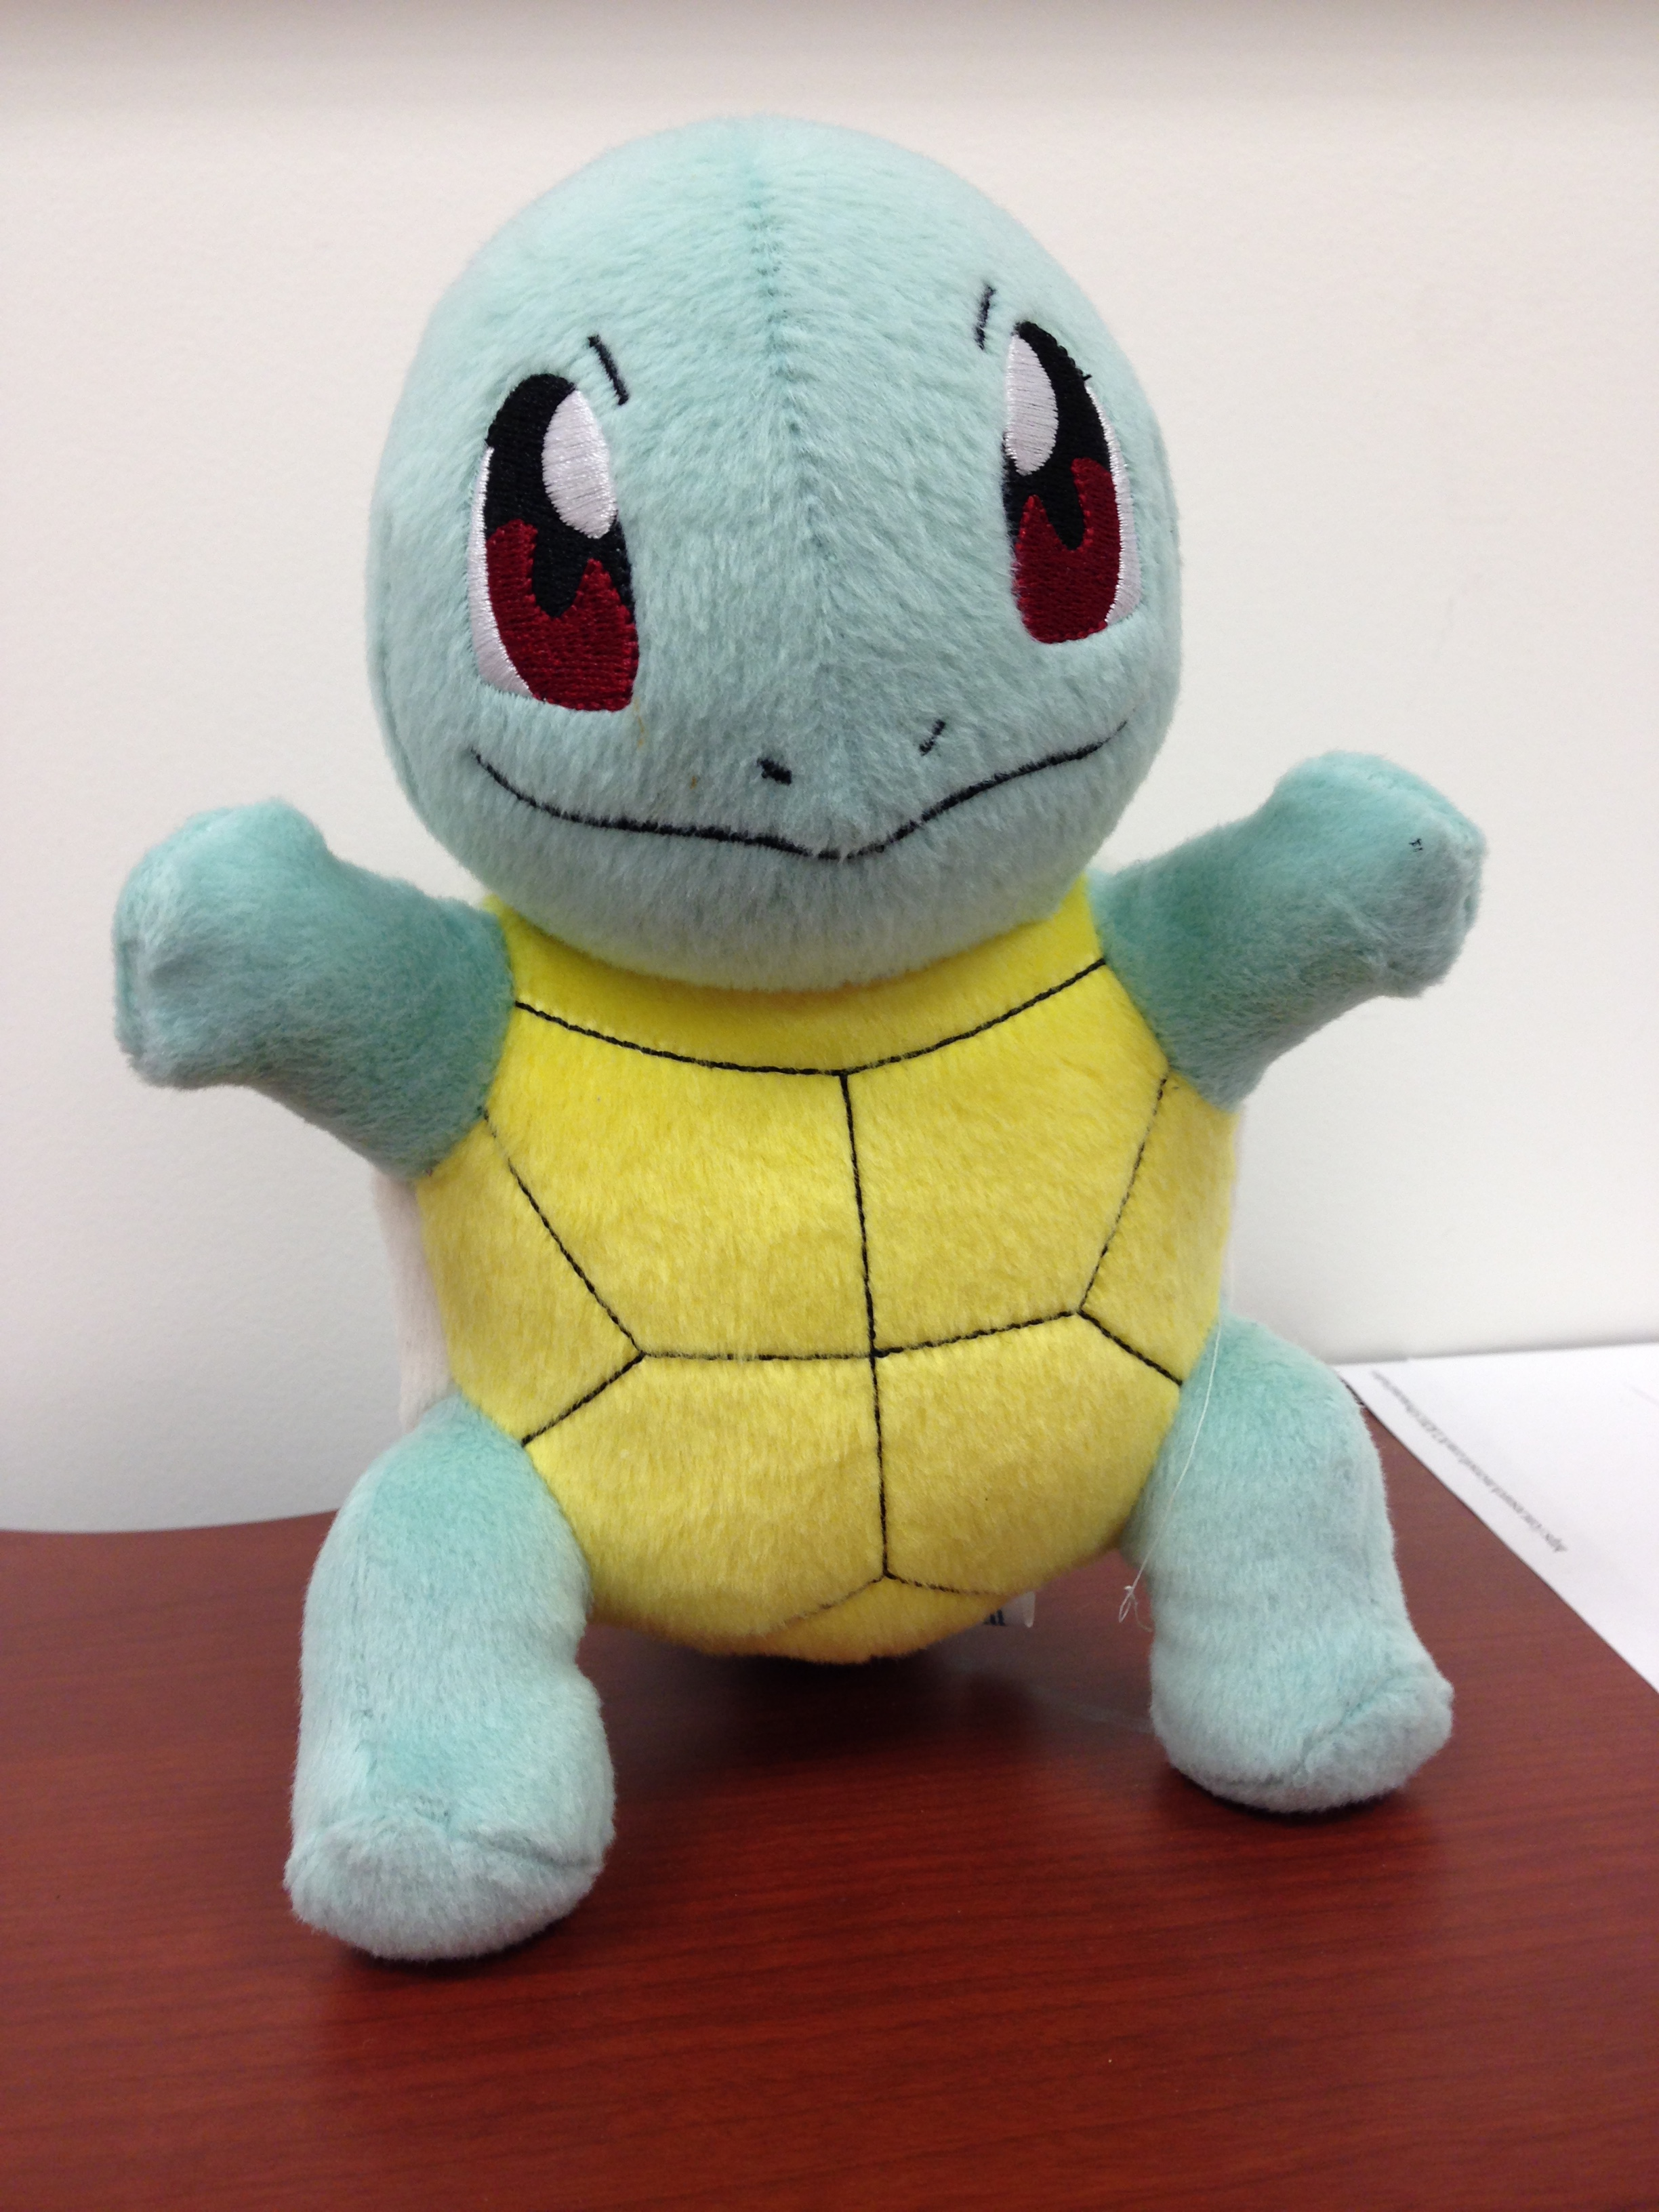
\includegraphics[width=\textwidth]{squirtle1.jpg}
		\caption{Left Image}
        \end{subfigure}
        \begin{subfigure}[b]{0.4\textwidth}
                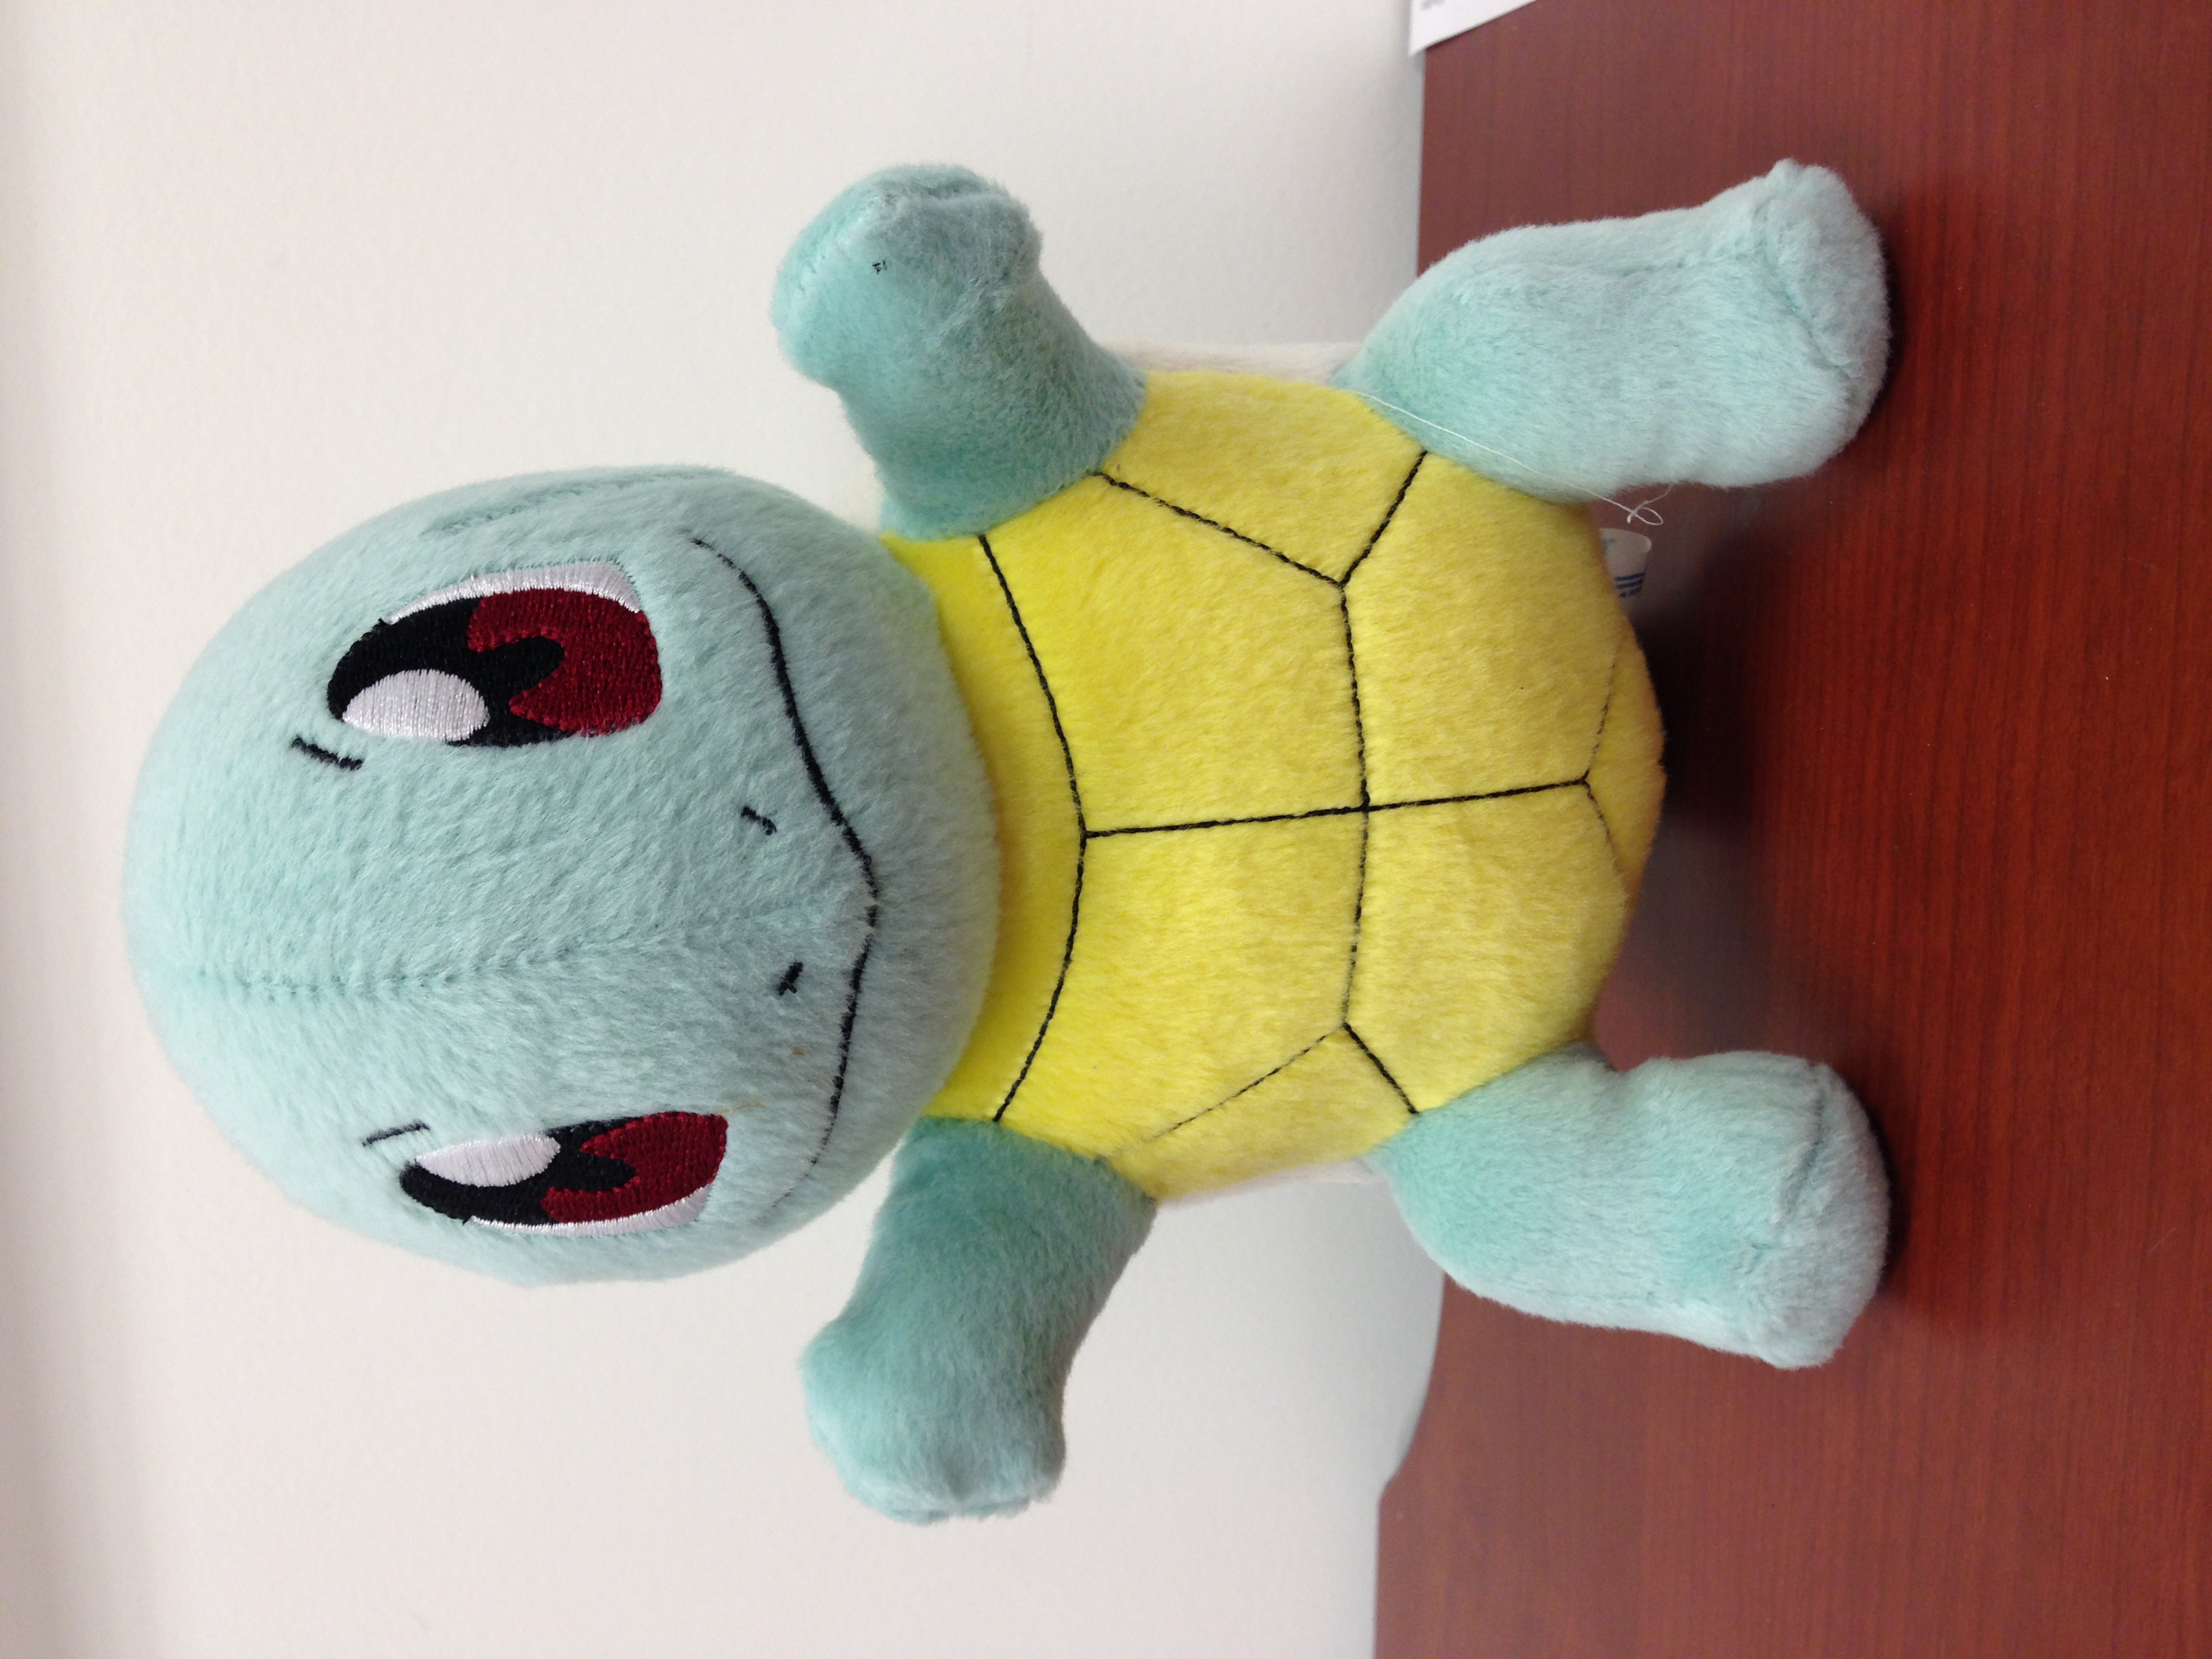
\includegraphics[width=\textwidth]{squirtle2.jpg}
                \caption{Right Image}
        \end{subfigure}
        \caption{Original Pictures of Stuffed Squirtle}
        \label{sq1}
\end{figure}

\begin{figure}[H]
\centering
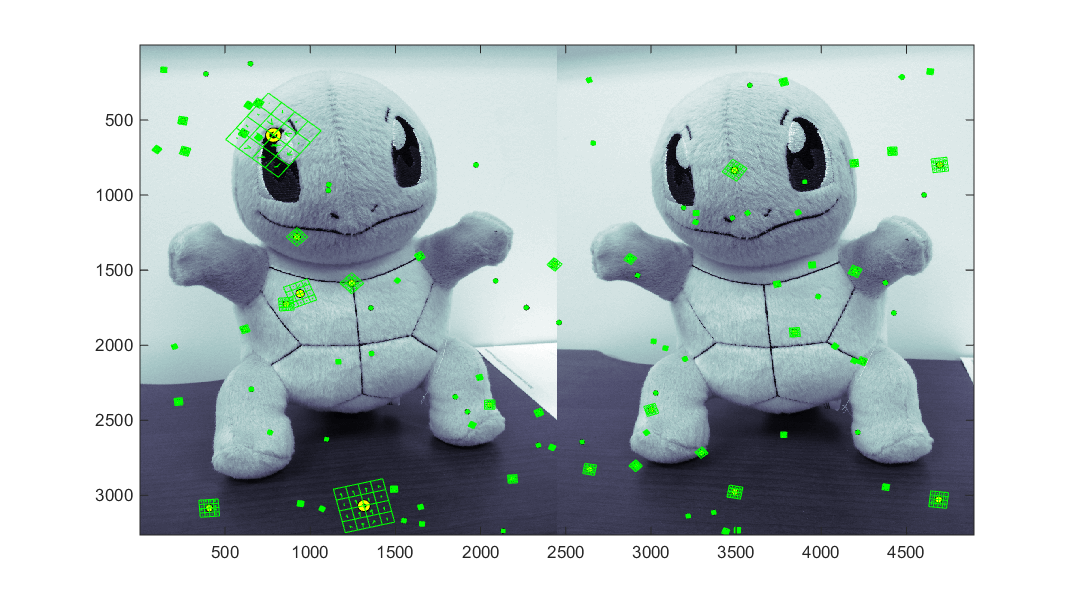
\includegraphics[height=3.5in]{squirtle_pointsWoMatching.png}
\caption{Squirtle Images With Points Marked}
\label{sq2}
\end{figure}

\begin{figure}[H]
\centering
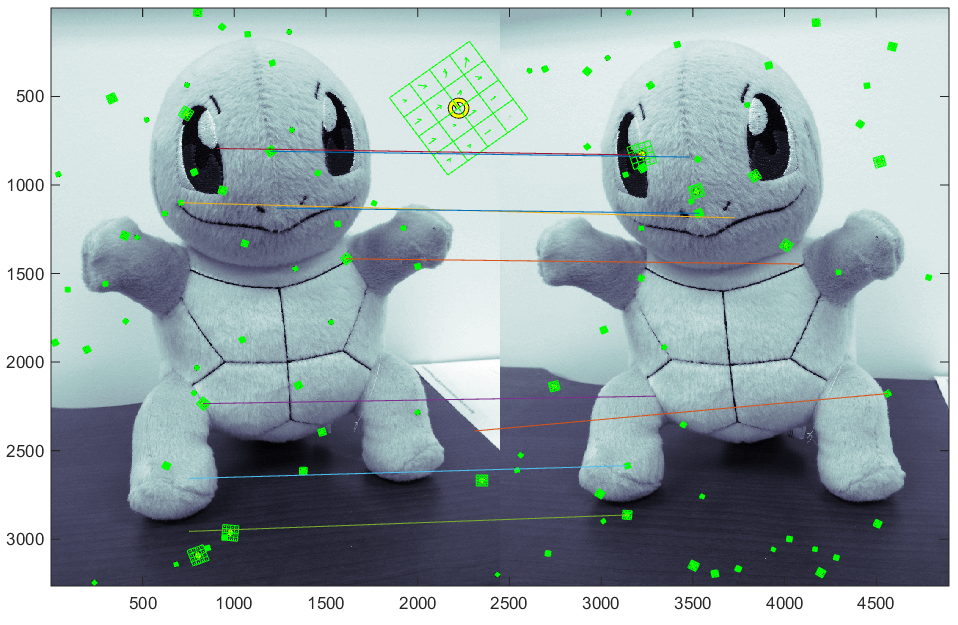
\includegraphics[height=3.5in]{squirtle_pointsWithMatching.png}
\caption{Squirtle Images With Points Marked and Some Matches Shown}
\label{sq3}
\end{figure}

\newpage

\subsection*{Book Example}

Figure \ref{bk1} shows the original pictures that I took of a textbook. Figure \ref{bk2} show 50 random points found by running SIFT. Figure \ref{bk3} shows some of the matches found using SIFT. 

\begin{figure}
        \centering
        \begin{subfigure}[b]{0.4\textwidth}
                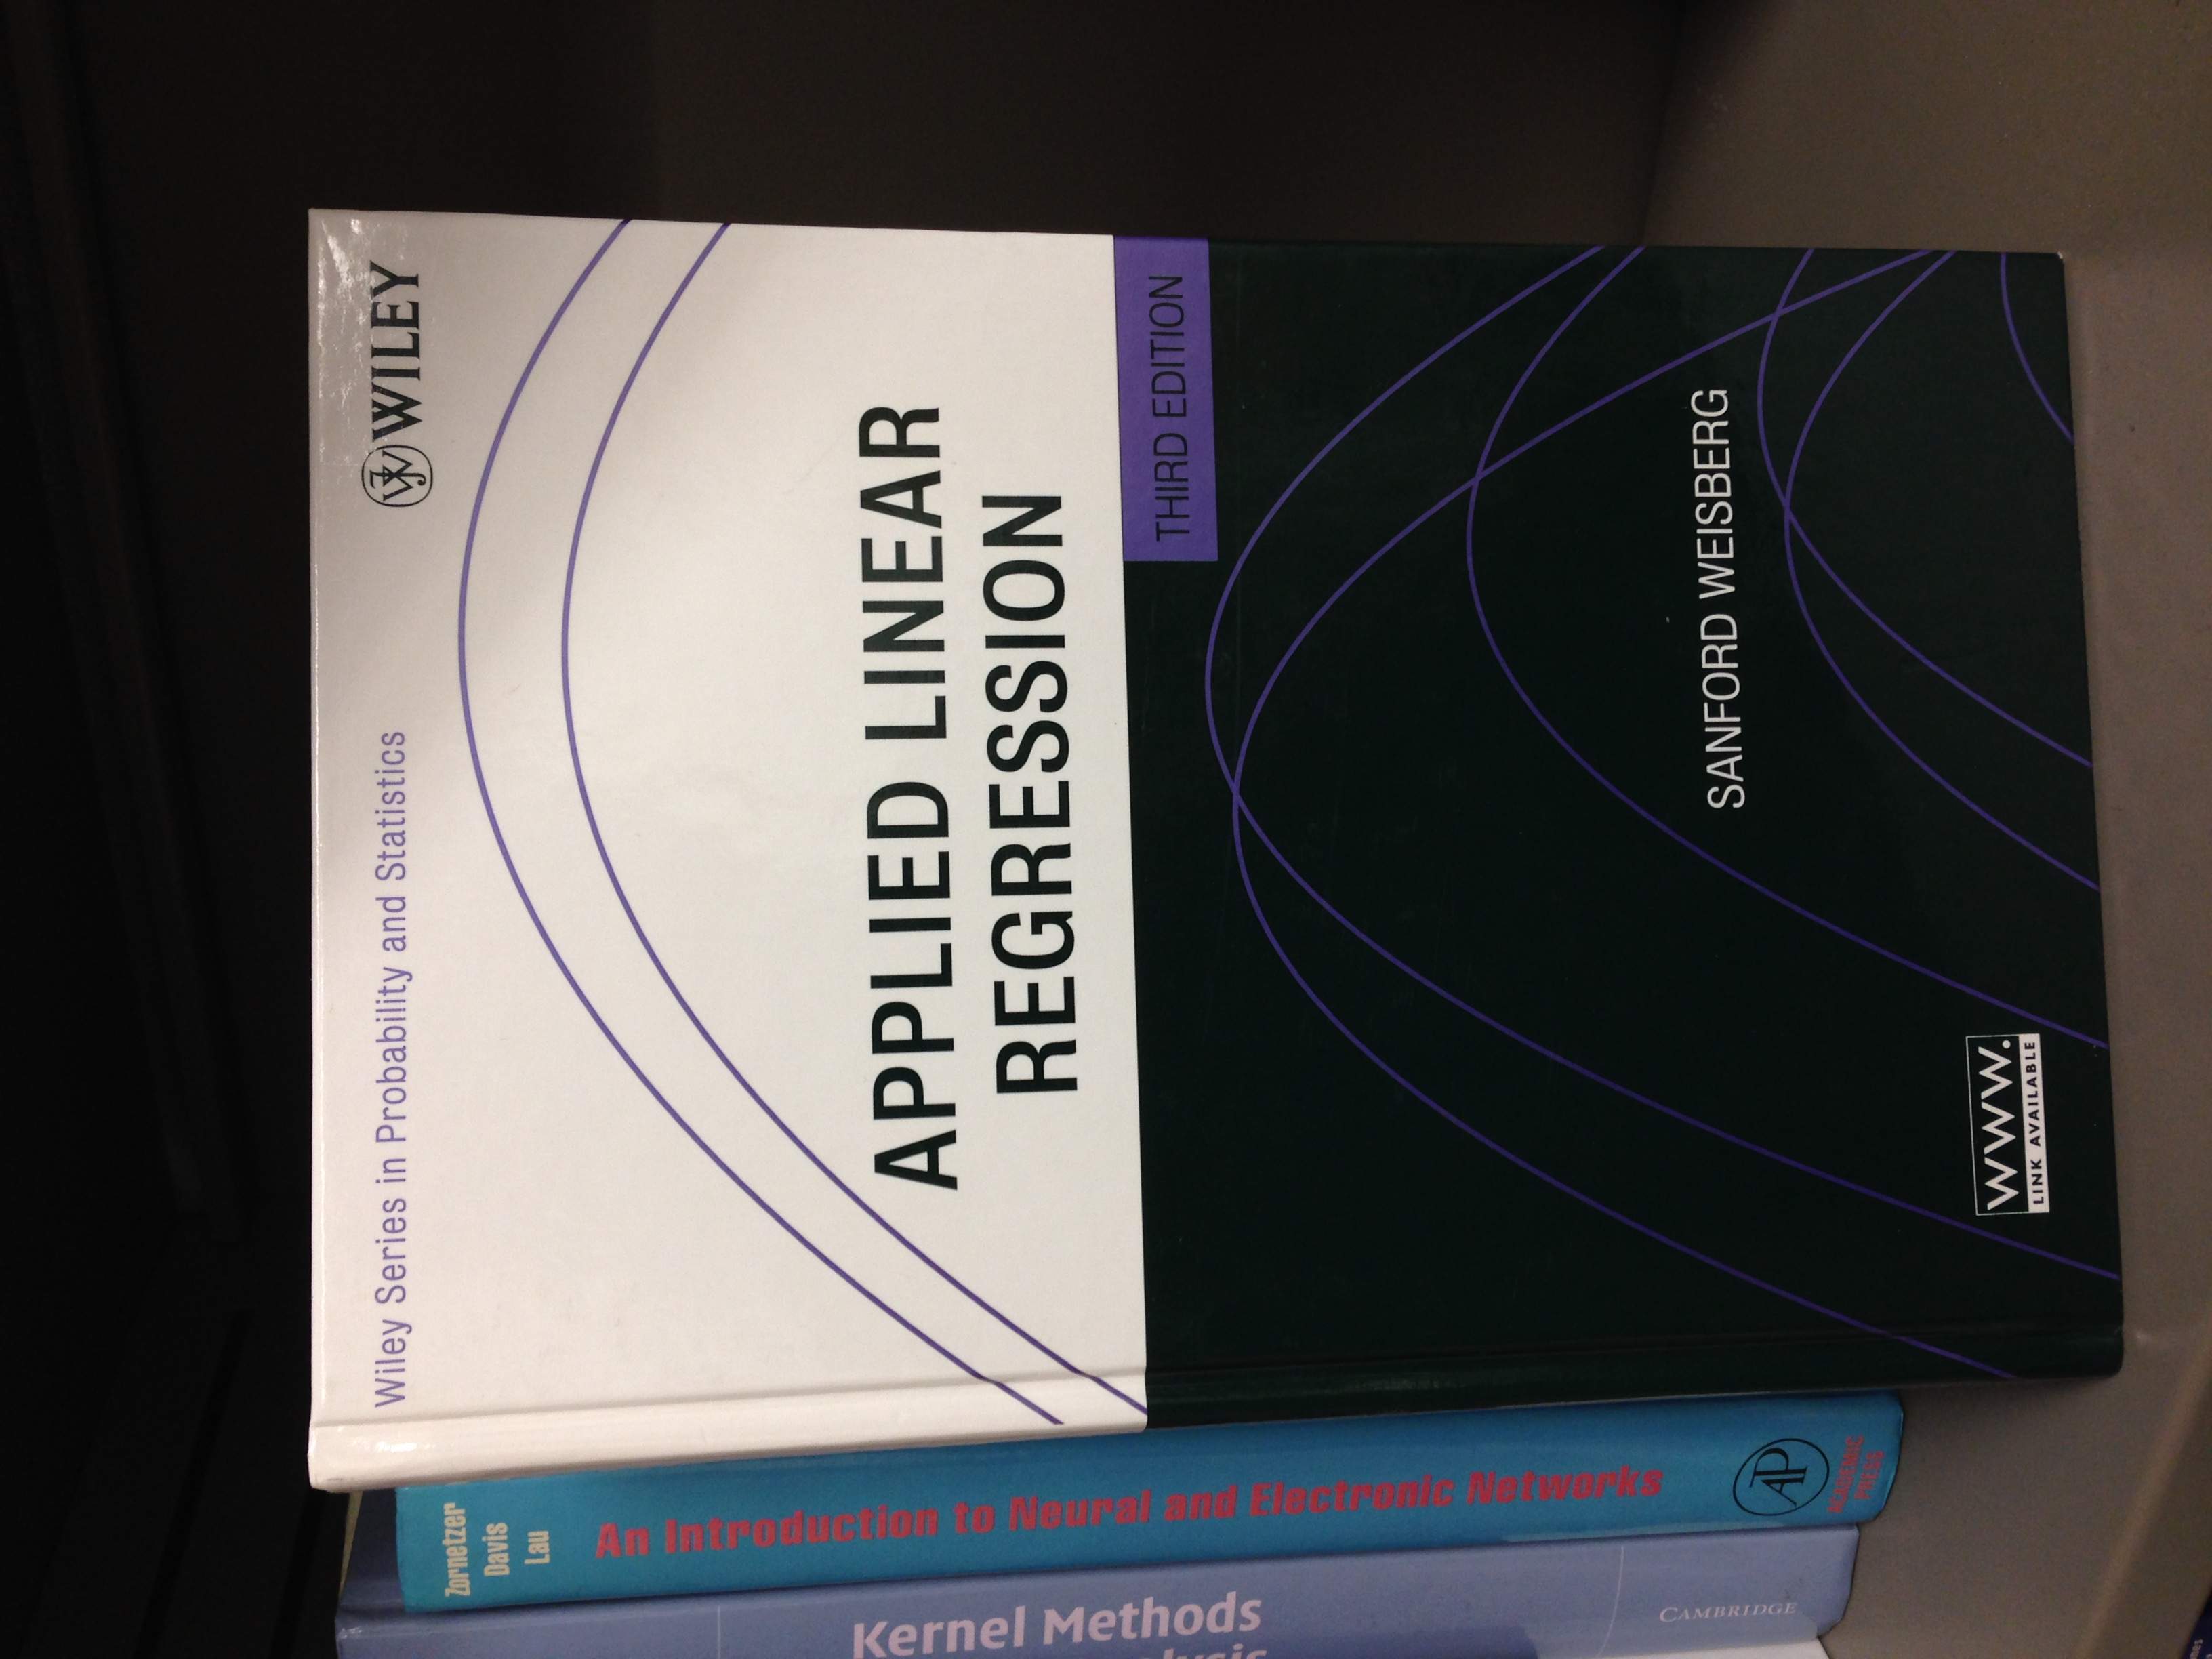
\includegraphics[width=\textwidth]{book1.jpg}
		\caption{Left Image}
        \end{subfigure}
        \begin{subfigure}[b]{0.4\textwidth}
                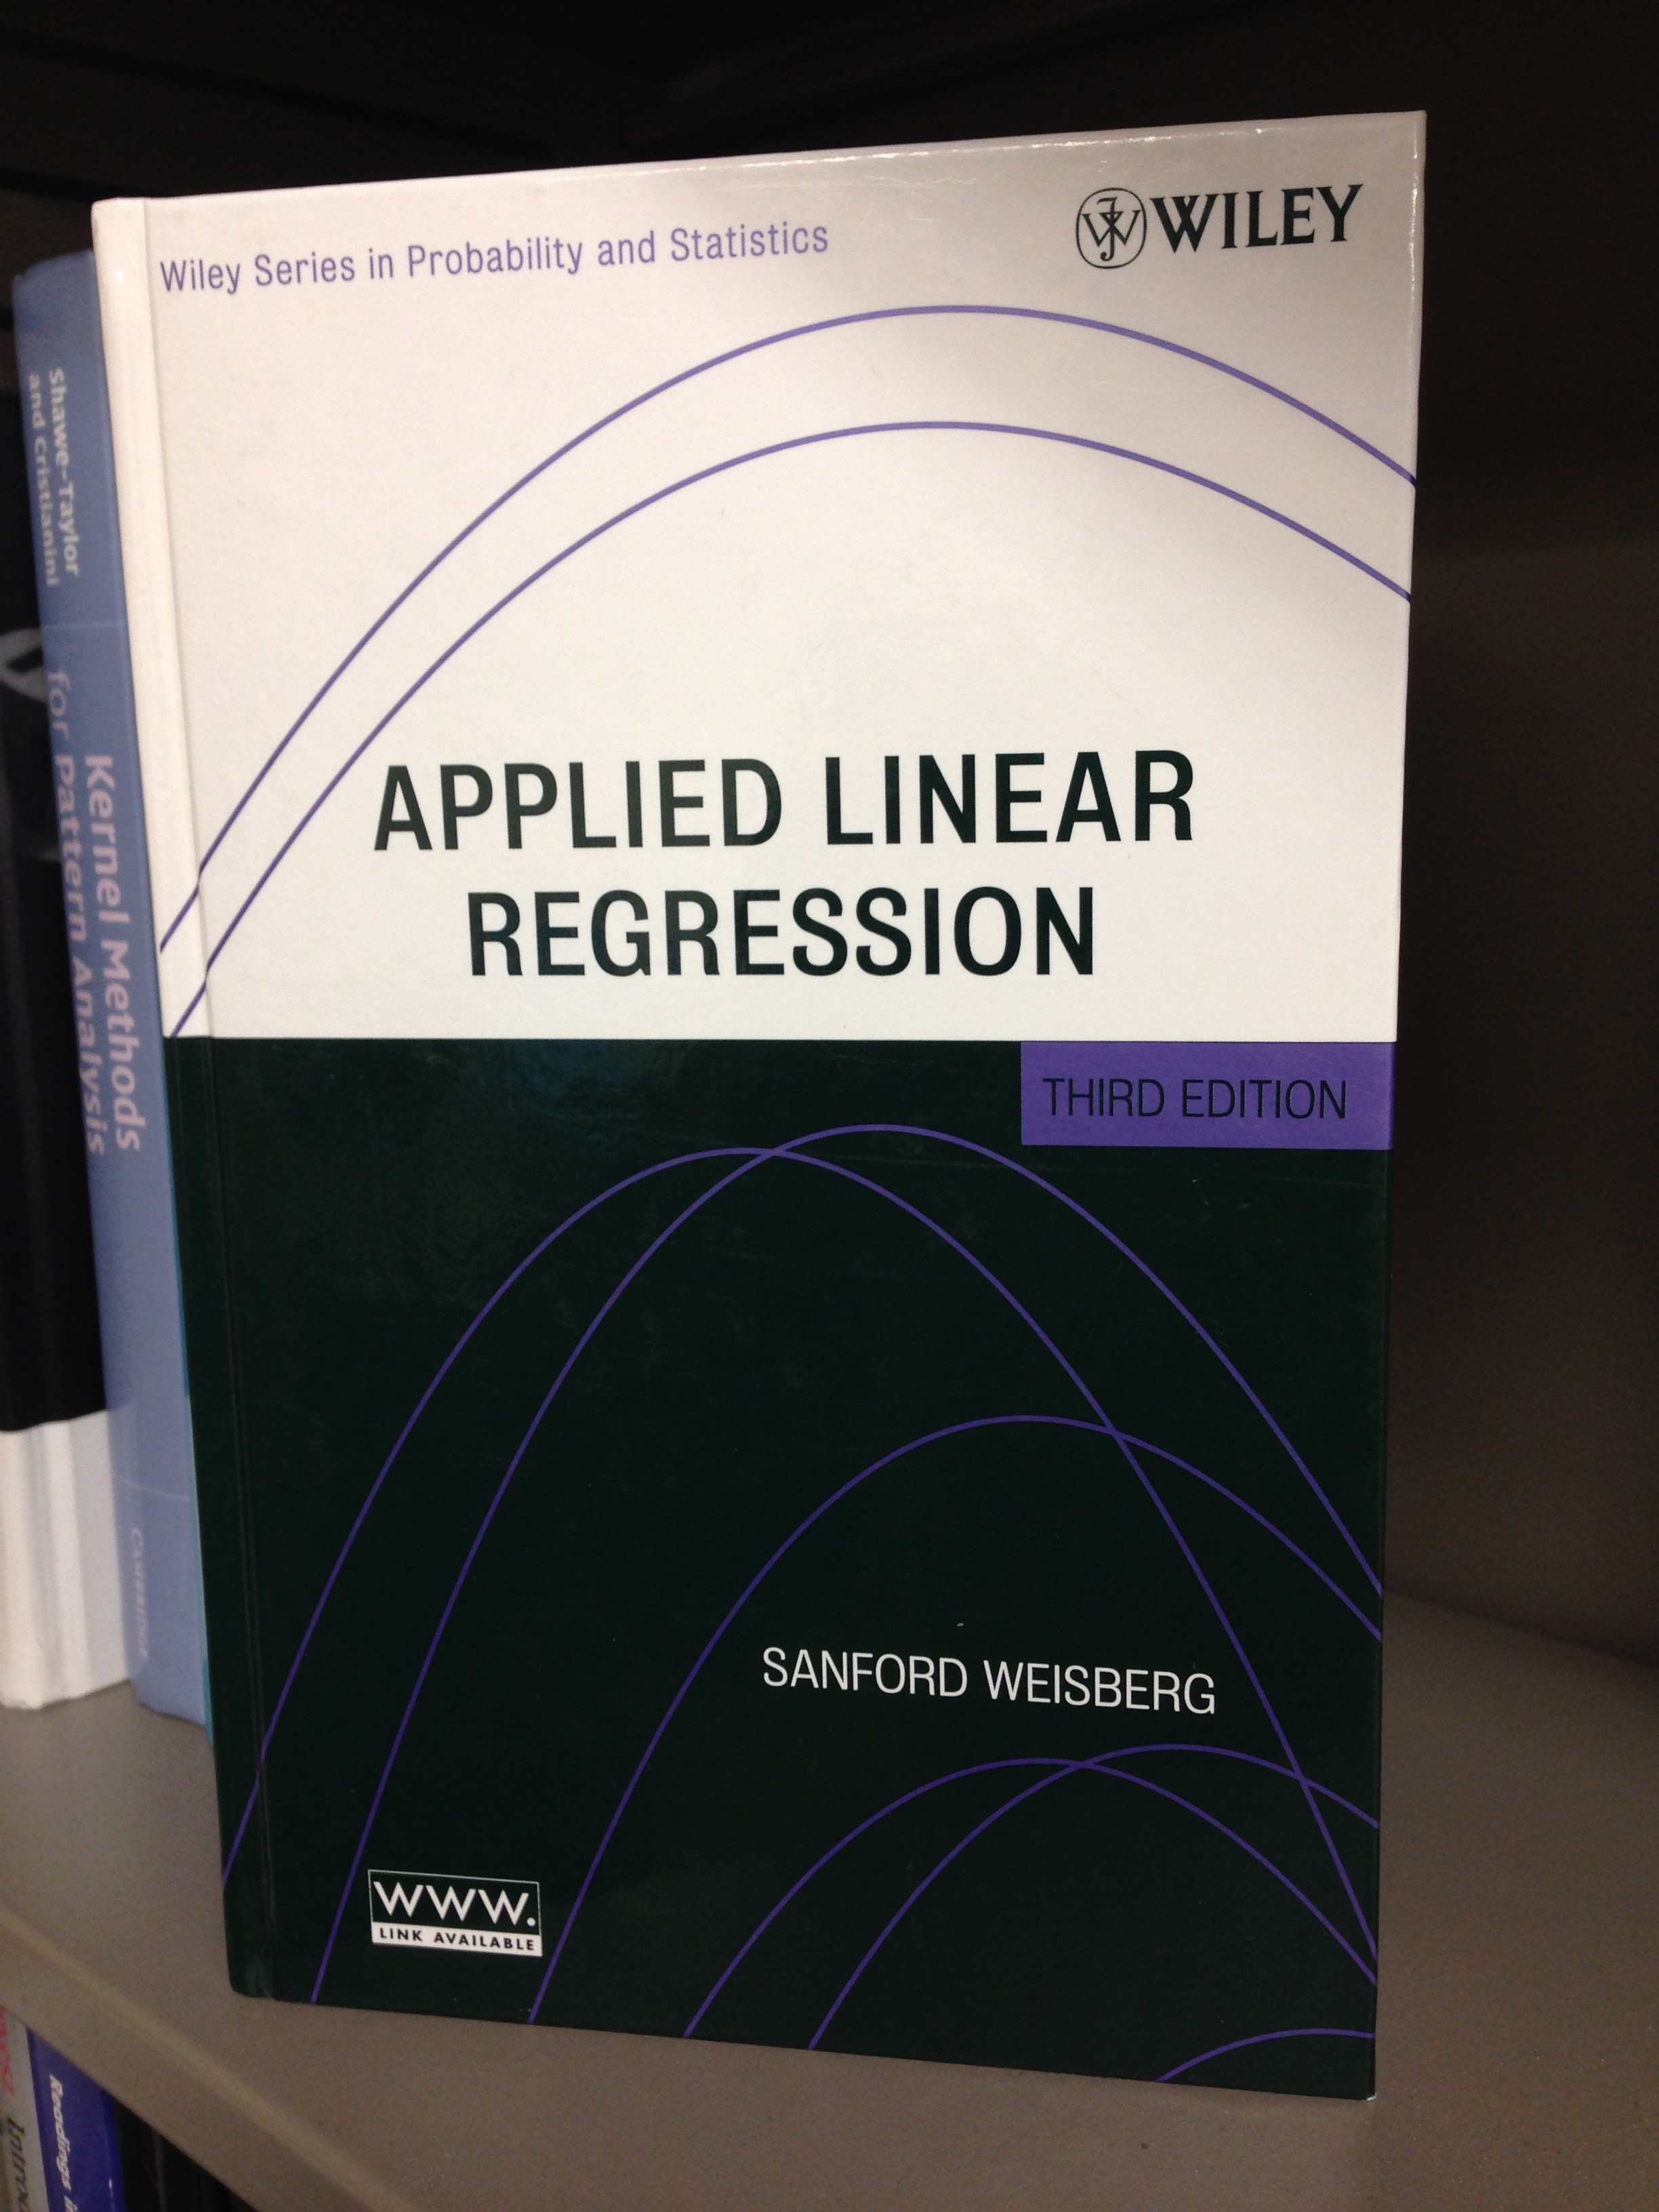
\includegraphics[width=\textwidth]{book2.jpg}
                \caption{Right Image}
        \end{subfigure}
        \caption{Original Pictures of Textbook}
        \label{bk1}
\end{figure}

\begin{figure}[H]
\centering
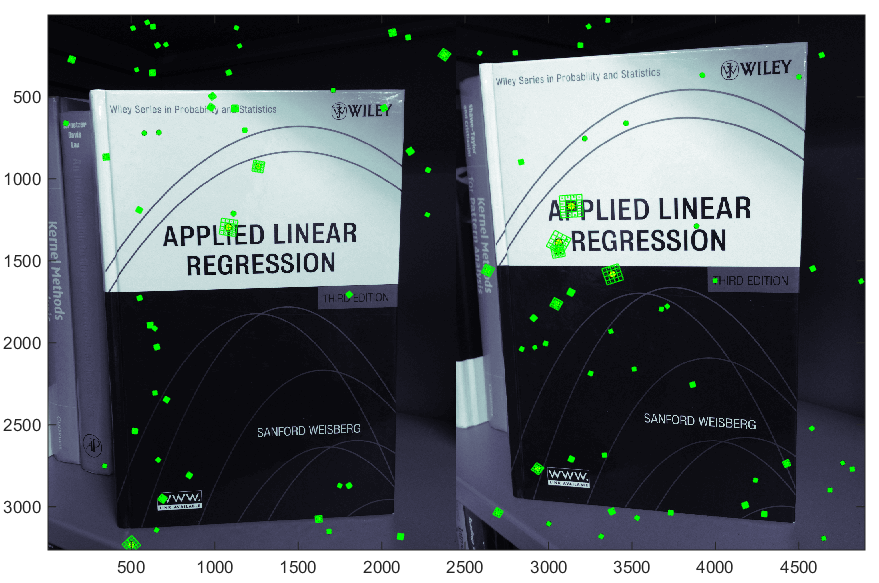
\includegraphics[height=3.5in]{book_pointsWoMatching.png}
\caption{Textbook Images With Points Marked}
\label{bk2}
\end{figure}

\begin{figure}[H]
\centering
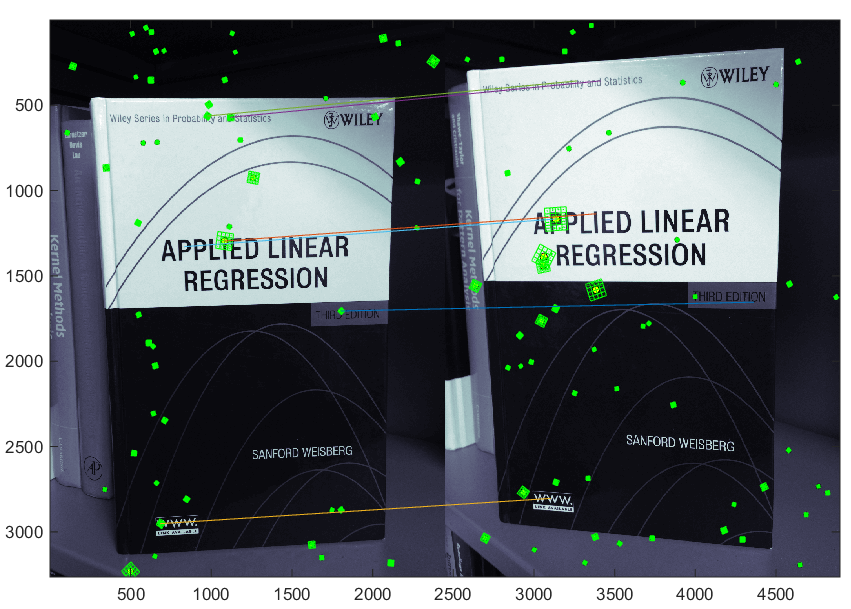
\includegraphics[height=3.5in]{book_pointsWithMatching.png}
\caption{Textbook Images With Points Marked and Some Matches Shown}
\label{bk3}
\end{figure}

\newpage

\subsection*{Coffee Can Example}

Figure \ref{cc1} shows the original pictures that I took of a coffee can. Figure \ref{cc2} show 50 random points found by running SIFT. Figure \ref{cc3} shows some of the matches found using SIFT. 

\begin{figure}
        \centering
        \begin{subfigure}[b]{0.4\textwidth}
                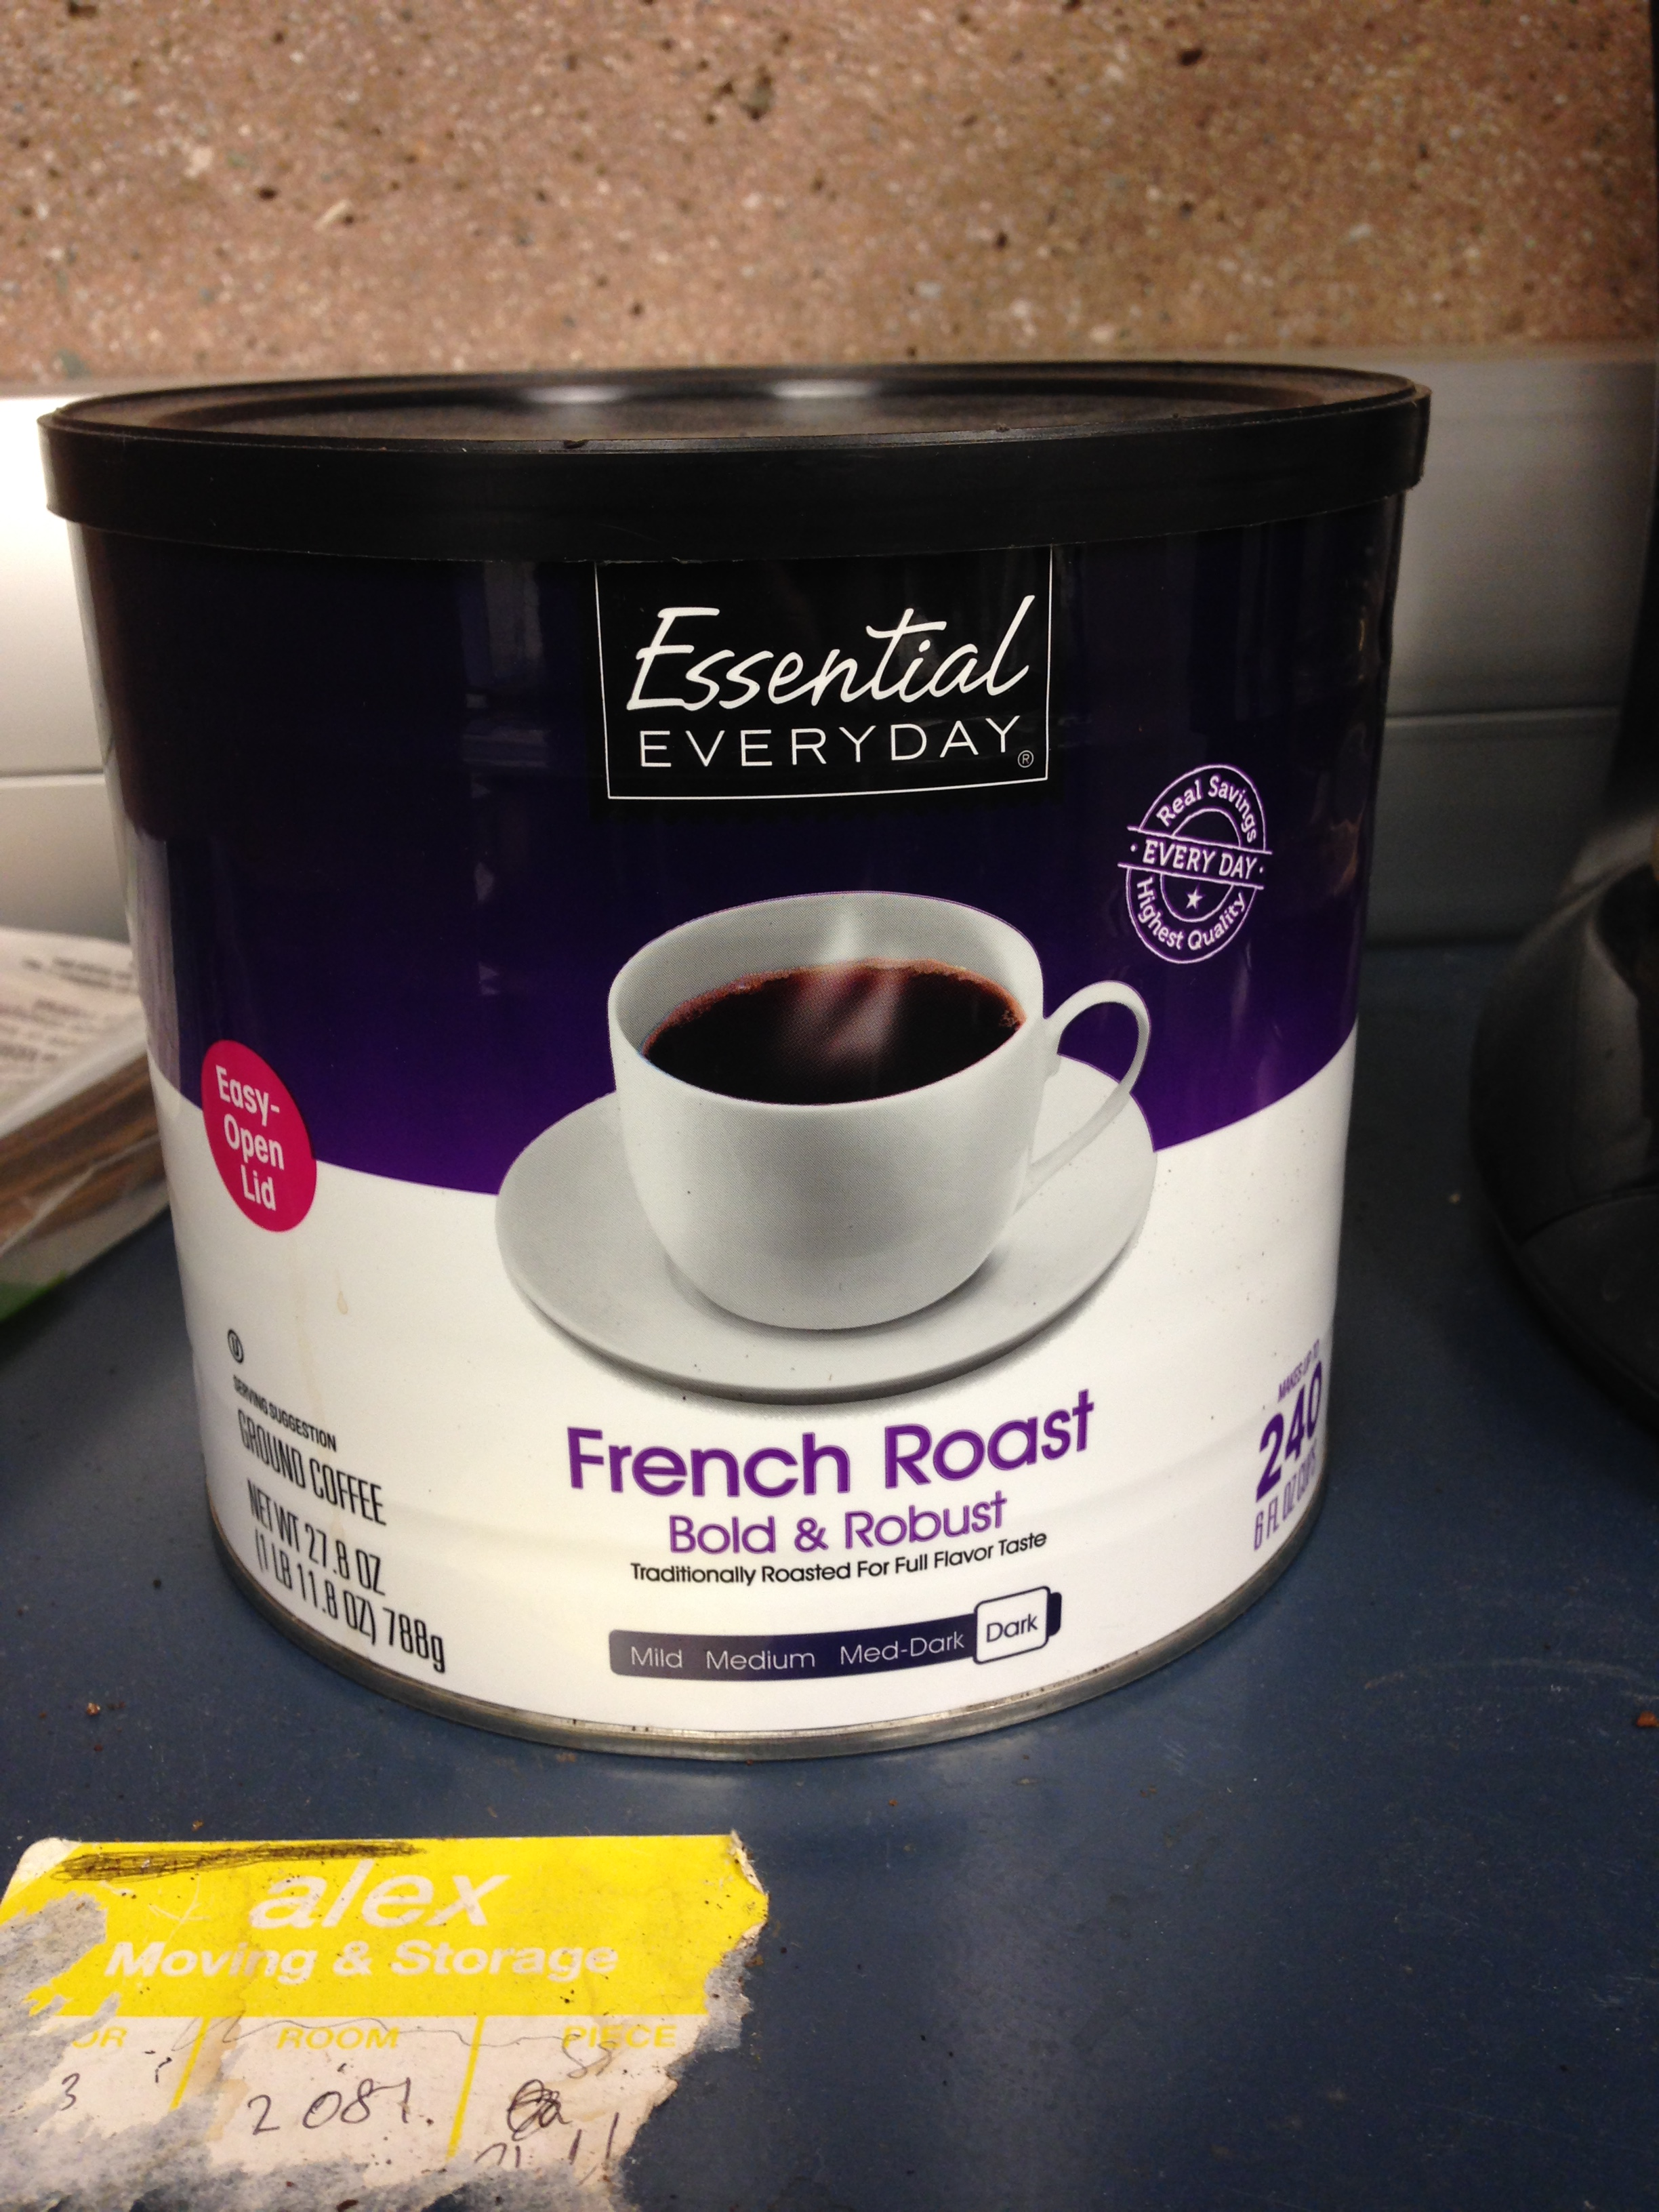
\includegraphics[width=\textwidth]{coffeeCan1.jpg}
		\caption{Left Image}
        \end{subfigure}
        \begin{subfigure}[b]{0.4\textwidth}
                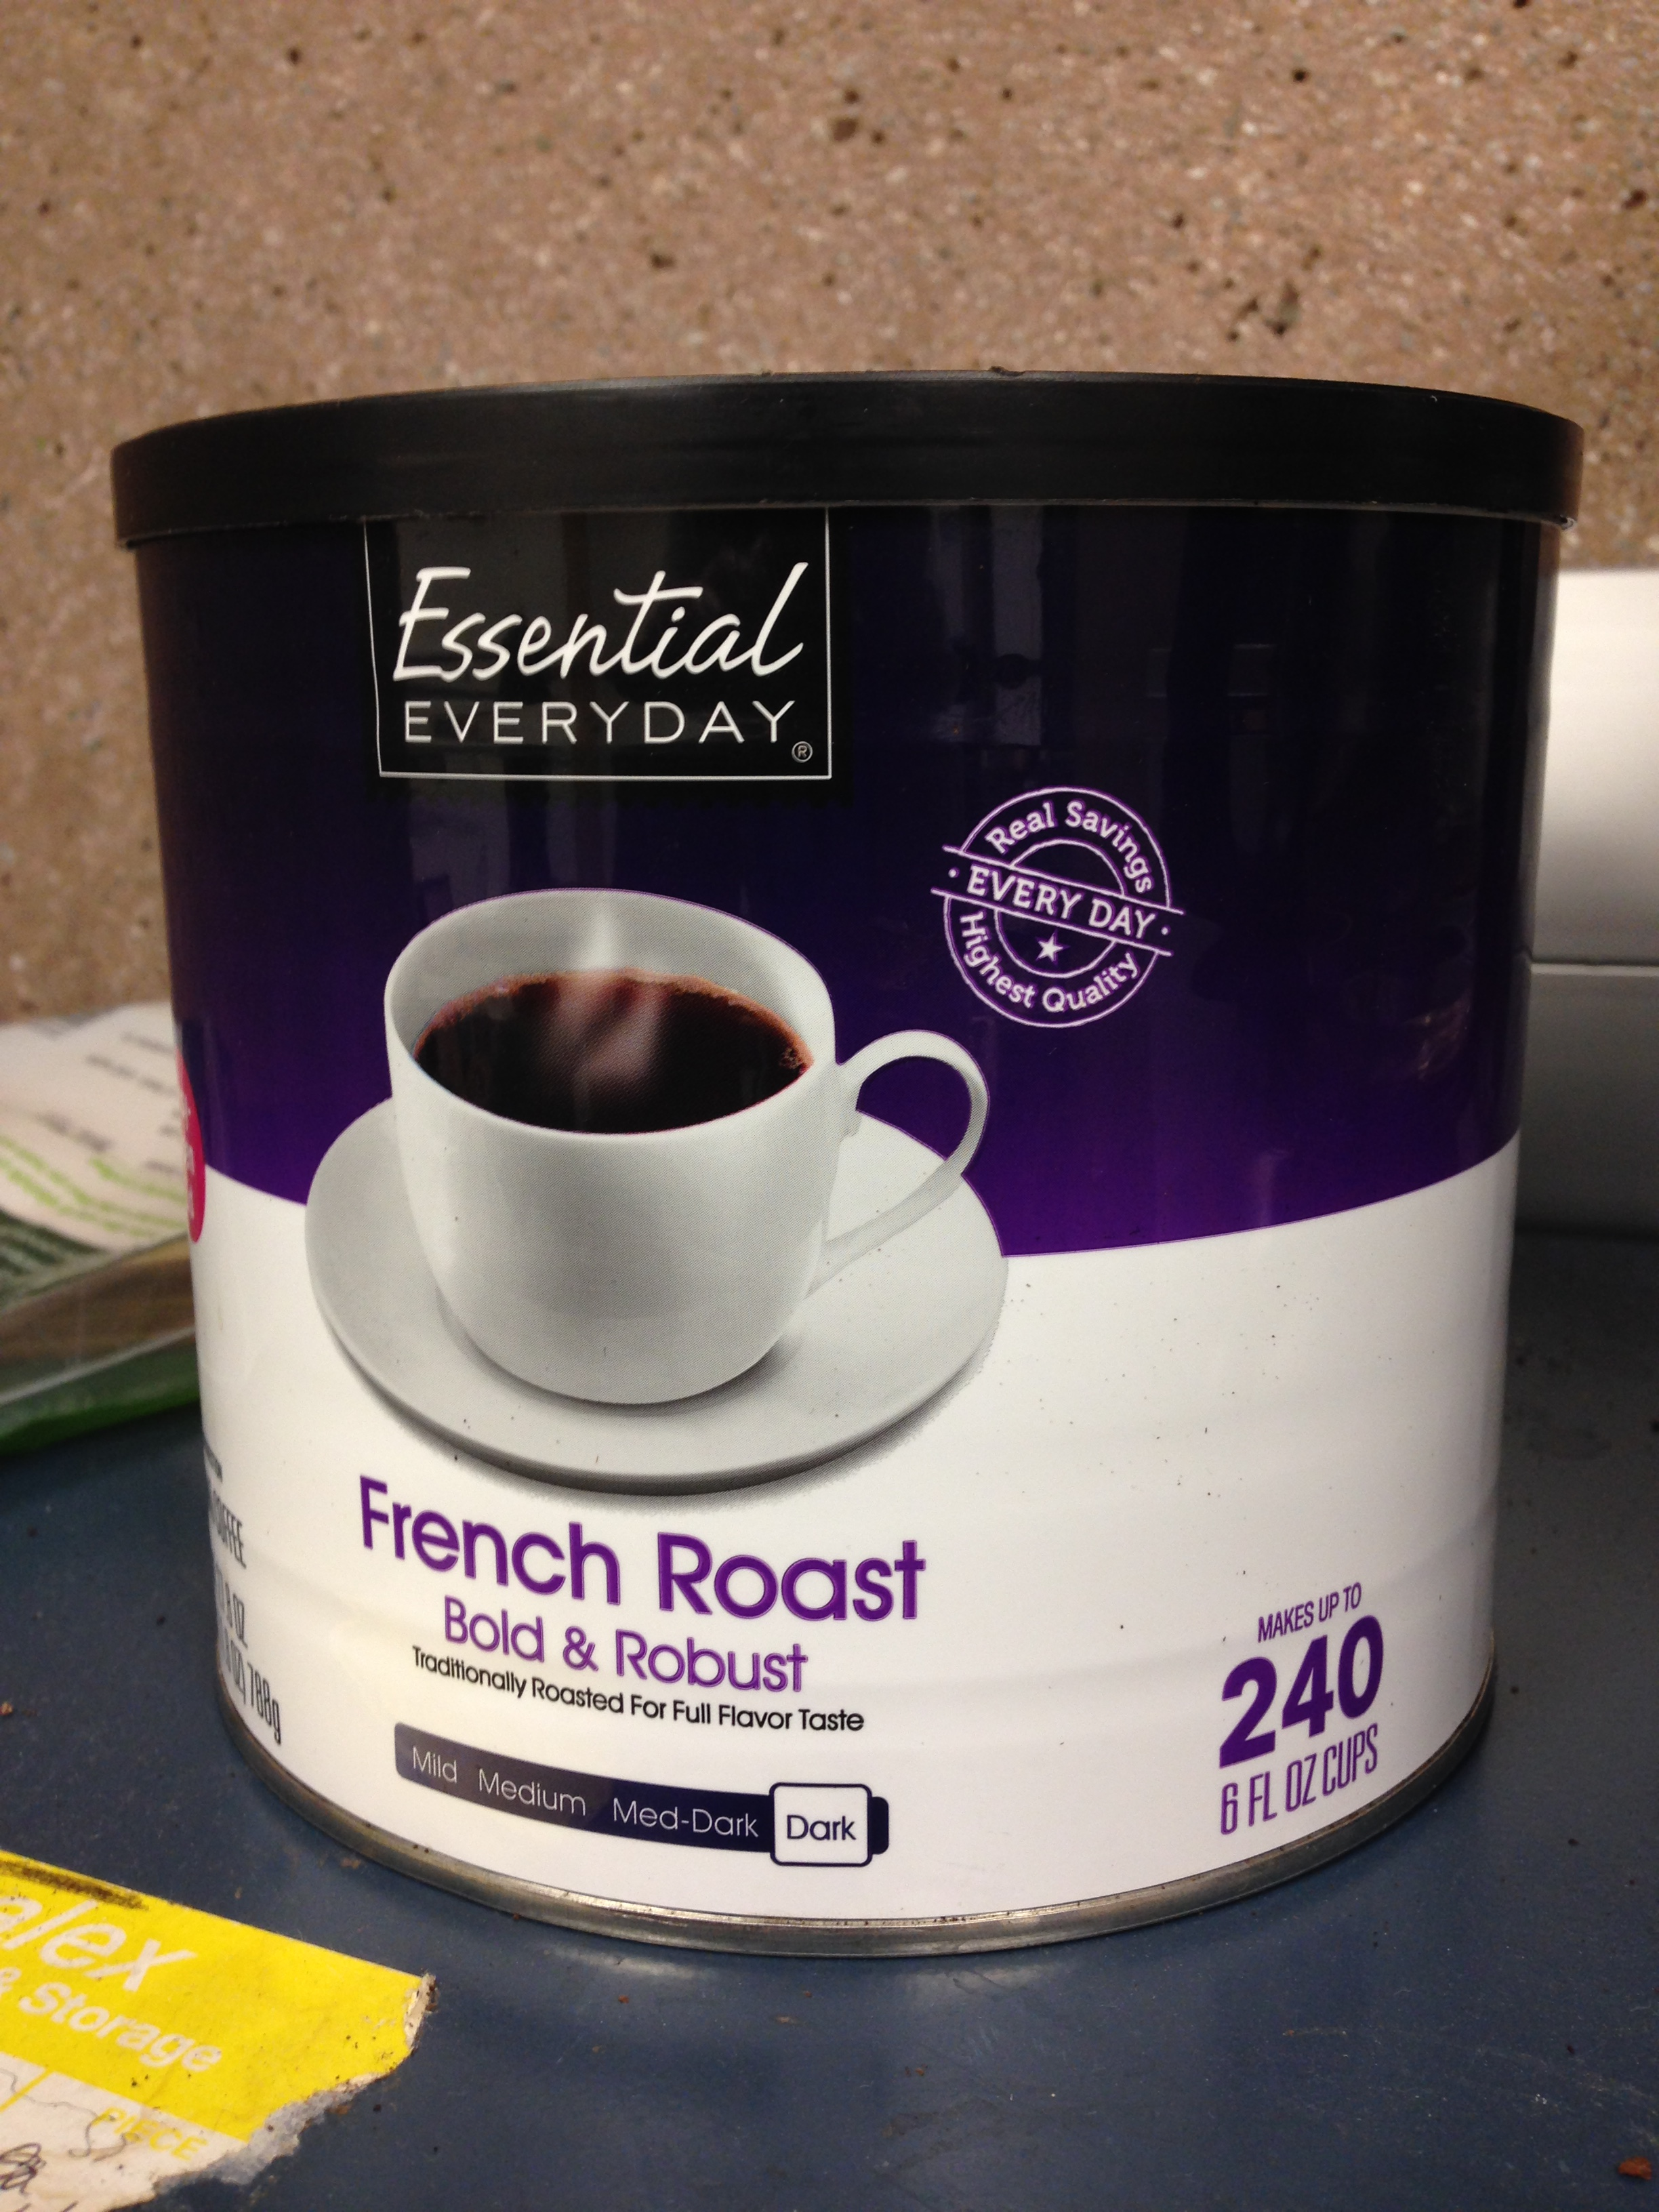
\includegraphics[width=\textwidth]{coffeeCan2.jpg}
                \caption{Right Image}
        \end{subfigure}
        \caption{Original Pictures of Coffee Can}
        \label{cc1}
\end{figure}

\begin{figure}[H]
\centering
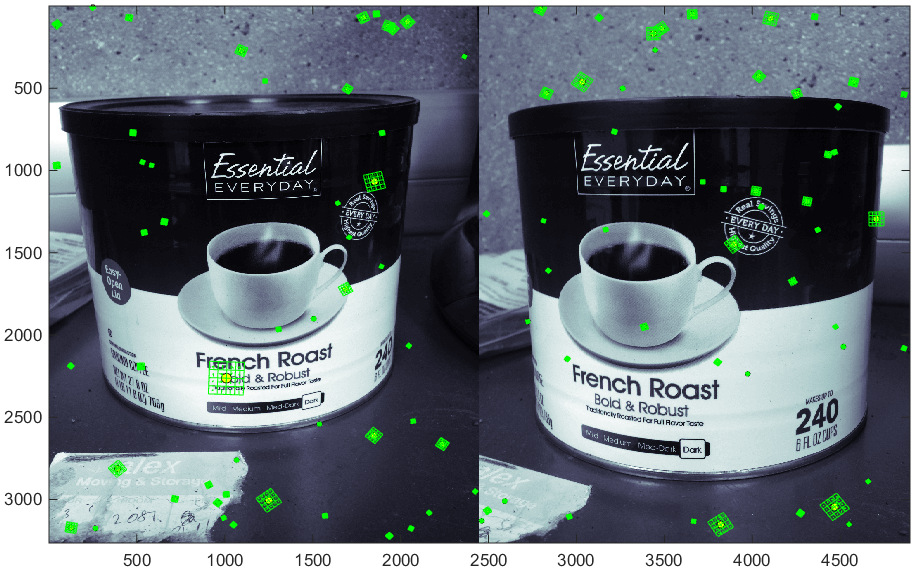
\includegraphics[height=3.5in]{coffeeCan_pointsWoMatching.png}
\caption{Coffee Can Images With Points Marked}
\label{cc2}
\end{figure}

\begin{figure}[H]
\centering
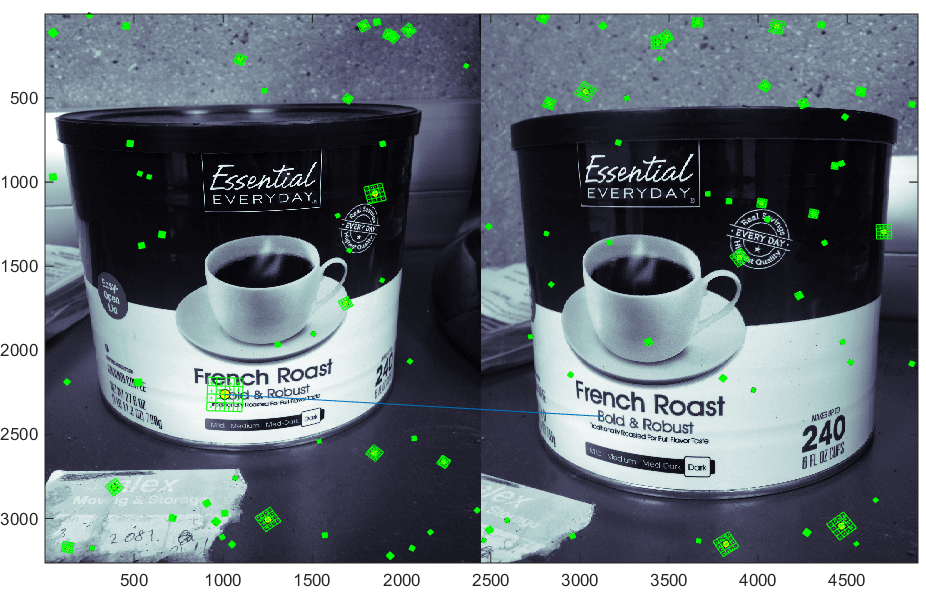
\includegraphics[height=3.5in]{coffeeCan_pointsWithMatching.png}
\caption{Coffee Can Images With Points Marked and Some Matches Shown}
\label{cc3}
\end{figure}

\newpage

\subsection*{Code for Problem 1}

Here is the code I used for this problem

\lstinputlisting[firstline=1, lastline=94]{prob1script.m}

\newpage

\section*{Problem 2}

\subsection*{Part A}

For problem 2, I used the same images as the previous problem but I chose my own points. Figures \ref{p2a},\ref{p2b}, and \ref{p2c} show the points that I chose in each image. After running my own implementation of RANSAC, I got the correspondences that are shown in figures \ref{p2d},\ref{p2e}, and \ref{p2f}

\begin{figure}[H]
\centering
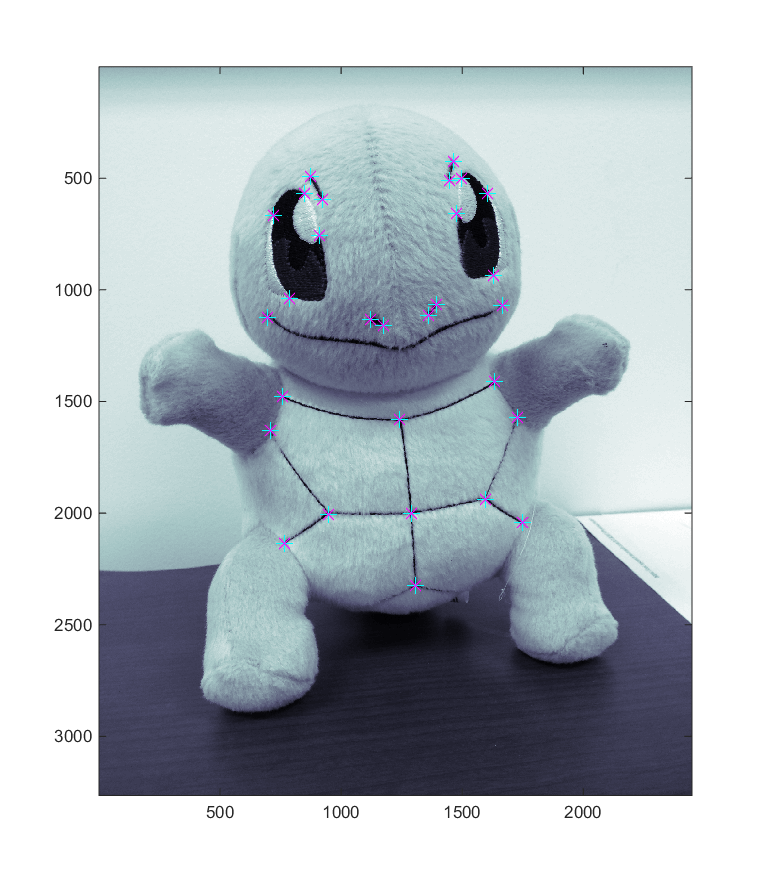
\includegraphics[height=7in]{squirtle_prob2Points.png}
\caption{Squirtle Image with Points Marked}
\label{p2a}
\end{figure}

\begin{figure}[H]
\centering
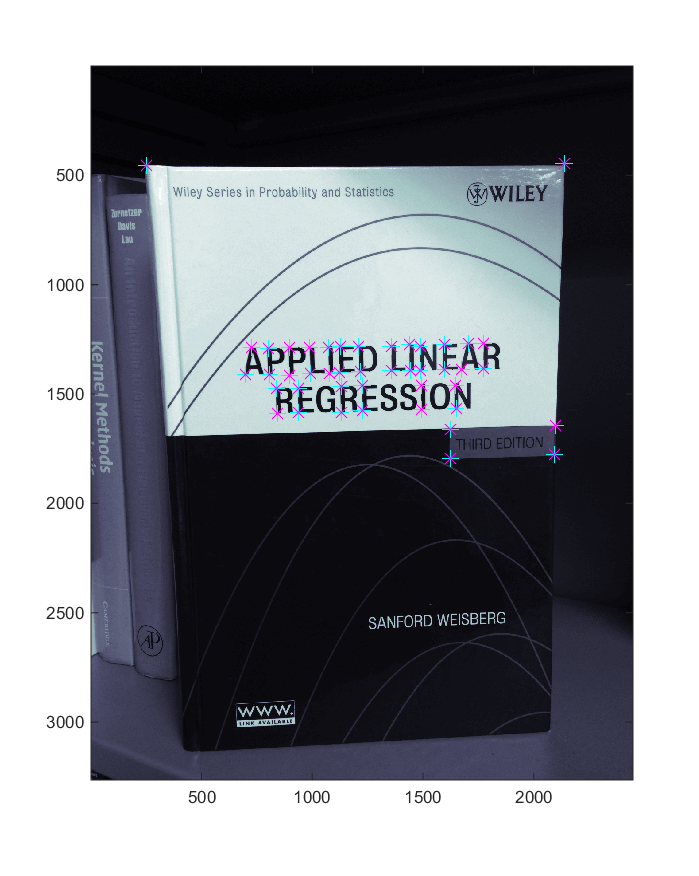
\includegraphics[height=7in]{book_prob2Points.png}
\caption{Textbook Image with Points Marked}
\label{p2b}
\end{figure}

\begin{figure}[H]
\centering
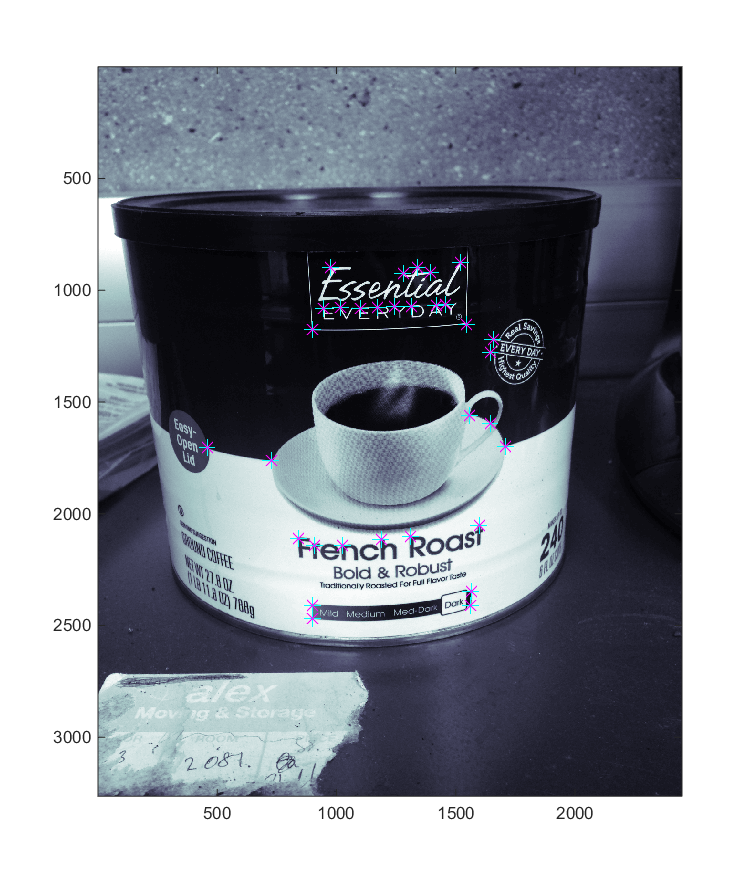
\includegraphics[height=7in]{coffeeCan_prob2Points.png}
\caption{Coffee Can Image with Points Marked}
\label{p2c}
\end{figure}

\begin{figure}[H]
\centering
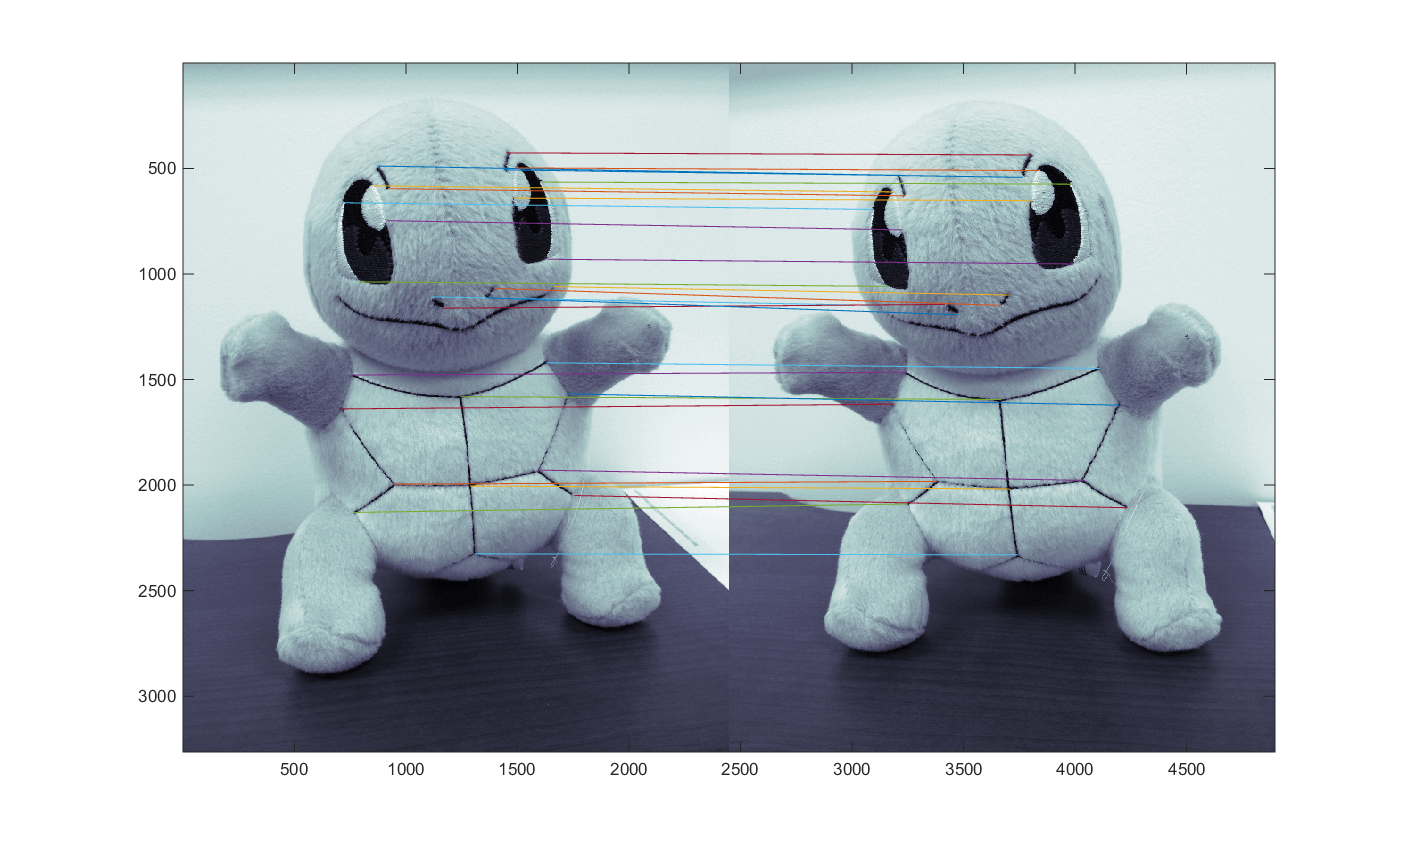
\includegraphics[height=5in]{squirtle_prob2Matches.png}
\caption{Squirtle Images with matching points}
\label{p2d}
\end{figure}

\begin{figure}[H]
\centering
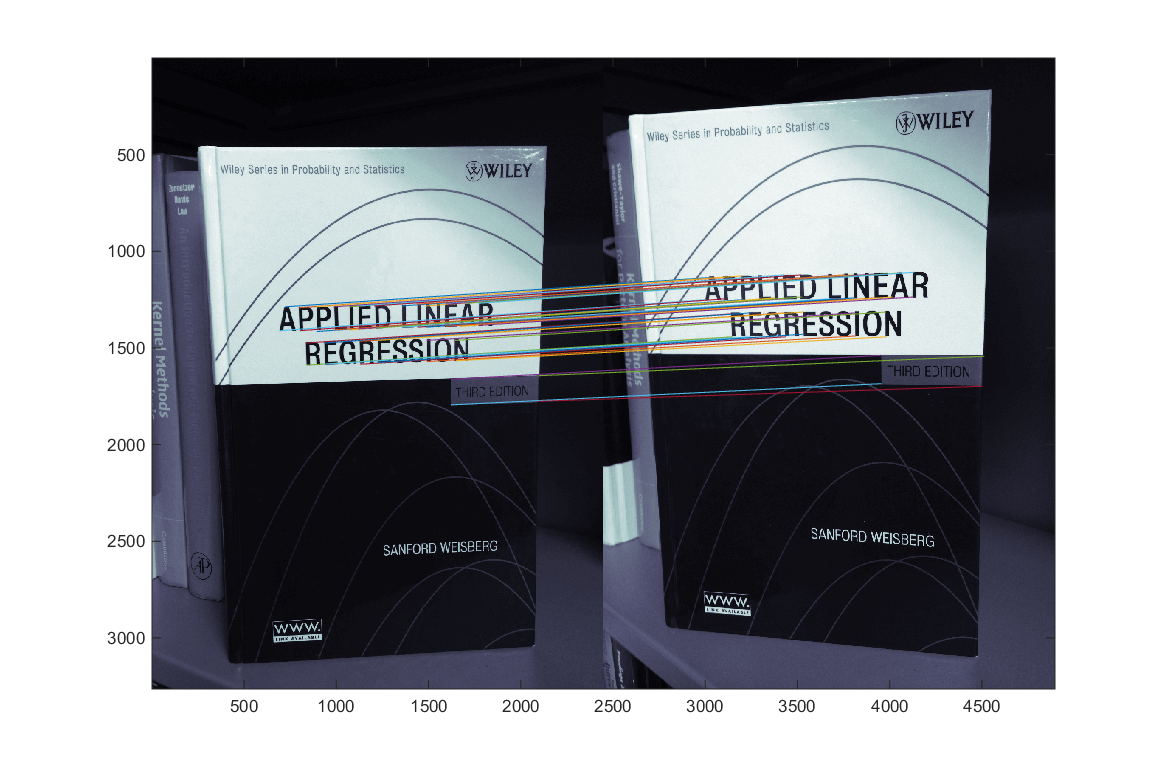
\includegraphics[height=5in]{book_prob2Matches.png}
\caption{Textbook Images with matching points}
\label{p2e}
\end{figure}

\begin{figure}[H]
\centering
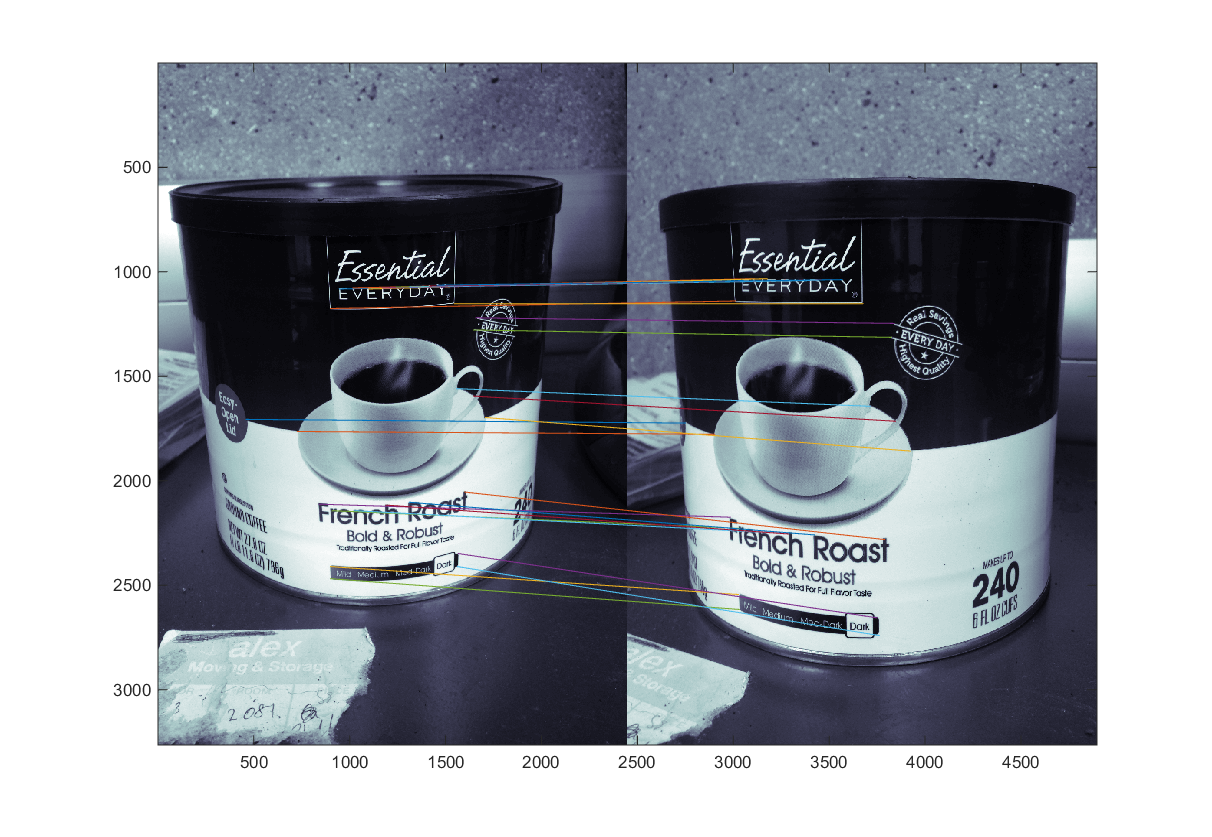
\includegraphics[height=5in]{coffeeCan_prob2Matches.png}
\caption{Coffee Can Images with matching points}
\label{p2f}
\end{figure}

\newpage

\subsection*{Part b}

With the squirtle image, the epipole for the left image lies slightly above the epipole for the right image, suggesting that the left image was taken from a slightly raised viewpoint as compared to the right image. With the coffee can image, the epipole of the left image is below the epipole for right image, suggesting that it was taken from a lowered viewpoint. 

\begin{figure}[H]
\centering
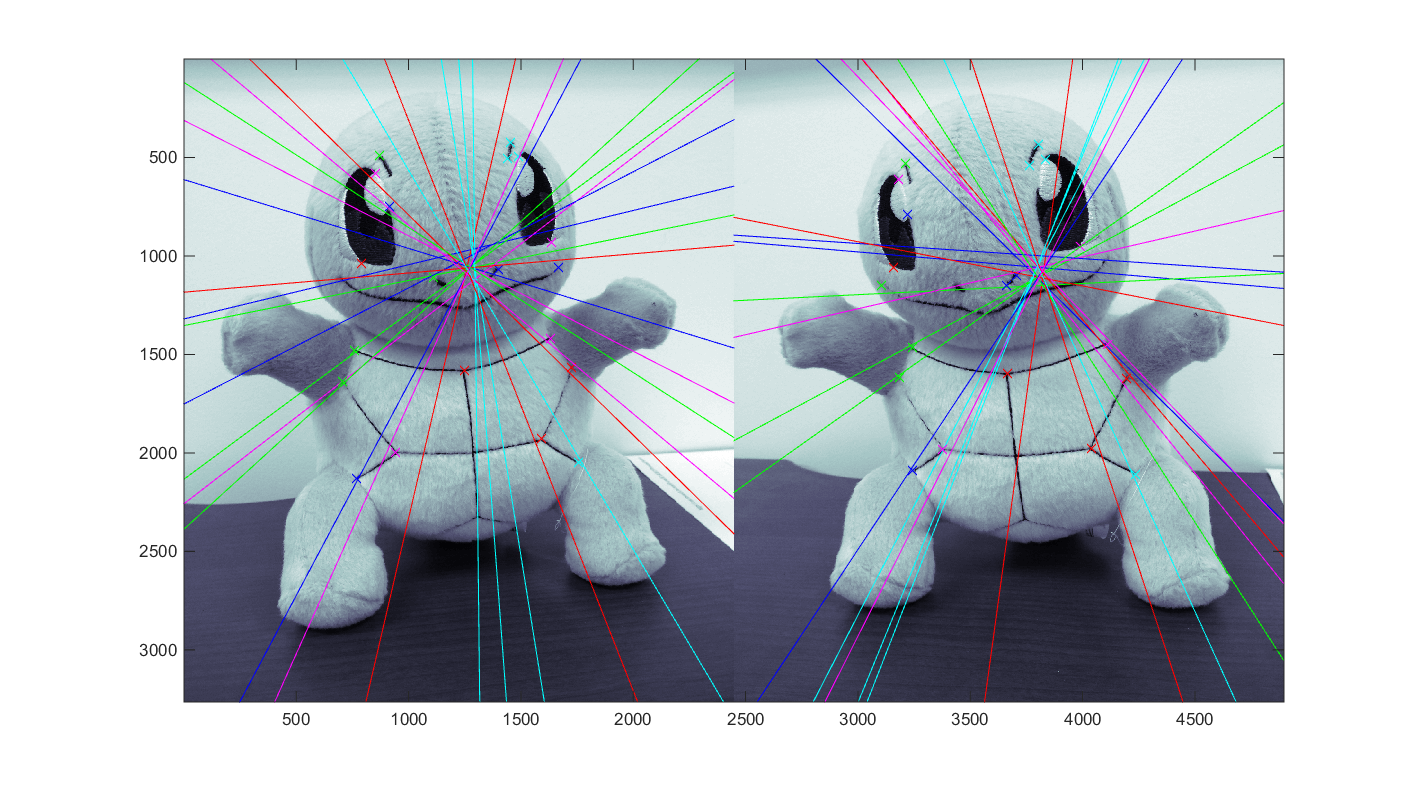
\includegraphics[height=3.5in]{squirtle_prob2Epipolar.png}
\caption{Squirtle Image with Epipolar Lines and their points}
\label{p2g}
\end{figure}

\begin{figure}[H]
\centering
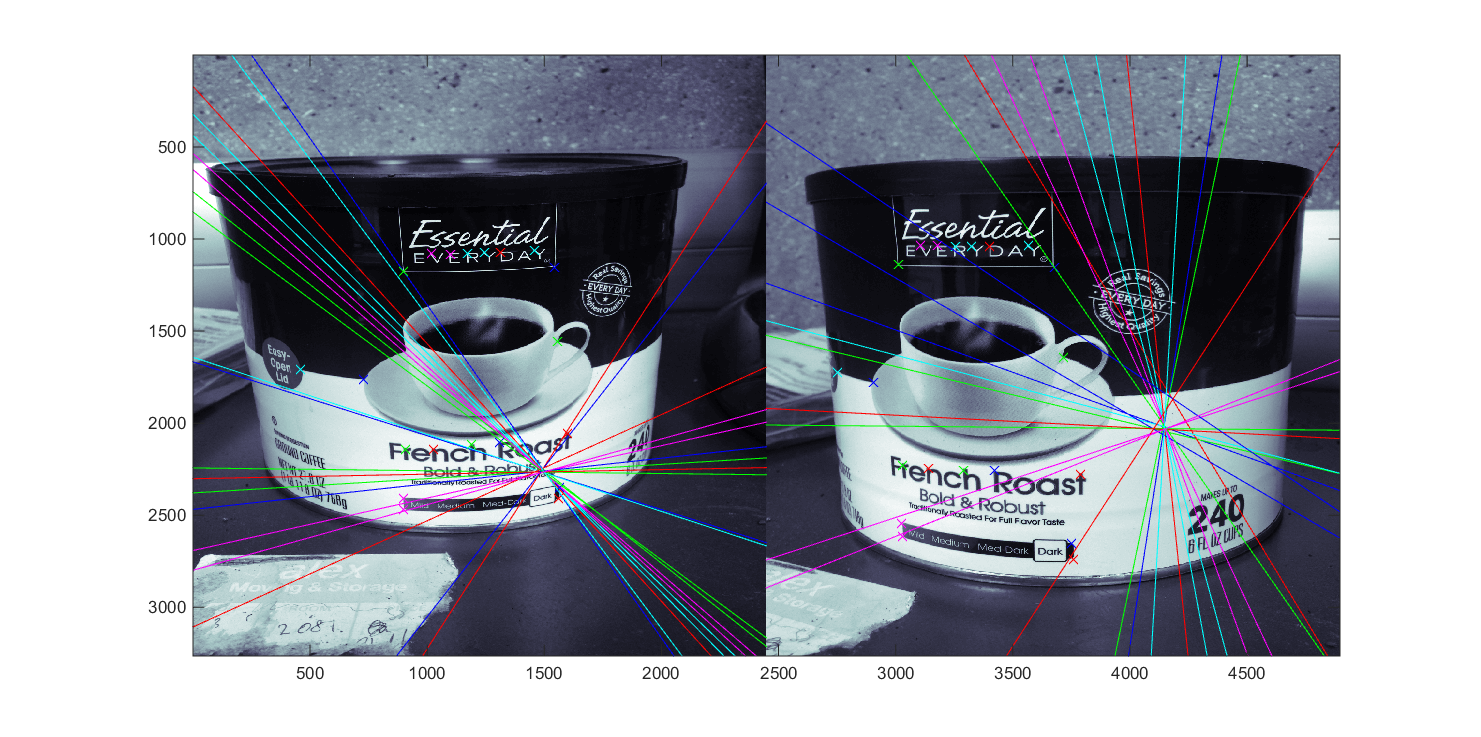
\includegraphics[height=3.5in]{coffeeCan_prob2Epipolar.png}
\caption{Coffee Can Image with Epipolar Lines and their points}
\label{p2h}
\end{figure}

\end{document}








